\documentclass[report2]{subfiles}

\begin{document}
\section{Circuit Description}
The keyboard encoder circuit takes a 64 bit input, and returns a 7 bit output. The 7 bit output represents the ascii code of the selected key, with each input line representing a single key. The codes are mapped from " " (space character, ascii 32) on the 0th input, to "\_" (underscore, ascii 95) on the 63rd input. \\
This ordering was chosen as the simplest conversion from key index to an appropriate ascii code. \\
\begin{center}
	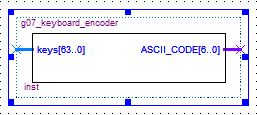
\includegraphics{keyboard_encode_symbol}
\end{center}
\subsection{Circuit Internal}
To actually create the circuit, a simple 64 to 6 bit encoder was used (which was in turn made of four 16 to 4 encoders from lab 1). The output of that circuit then had 32 added to it, to shift the result to an appropriate ascii code.

\end{document}